\appendix
\chapter{Additional Figures for Metric Trends on Different Algorithms}
\label{app:sep_trends_per_algo}
In this appendix, we add the Figures that we omitted in Section \ref{subsec:trends_datasets}, were we fit a line of best fir per algorithm per dataset in the scatterplots of the metrics for different utility measures. We see that per dataset, the trends are not always consistent, providing another argument as to why metrics do not have much value as general utility measuring tools.

\begin{figure}[!ht]
    \centering
    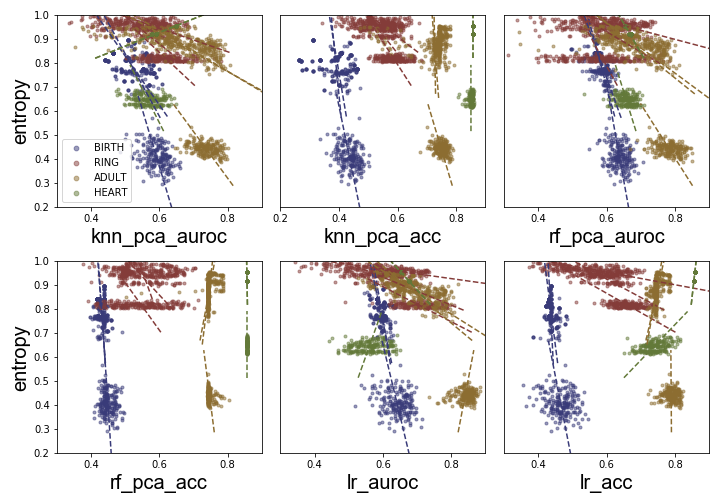
\includegraphics[width=0.8\textwidth]{project/fig/scatter_sep_trends/entropy_scatter.png}
    \caption{Scatterplots of the utility measures for the different classifiers against the entropy metric, separated by datasets. For every dataset, we draw a line of best fit per algorithm.}
\end{figure}

\begin{figure}[!ht]
    \centering
    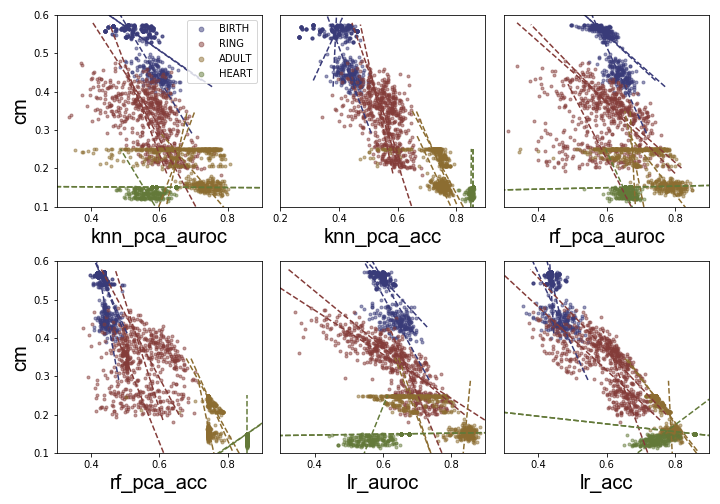
\includegraphics[width=0.8\textwidth]{project/fig/scatter_sep_trends/cm_scatter.png}
    \caption{Scatterplots of the utility measures for the different classifiers against the classification metric, separated by datasets. For every dataset, we draw a line of best fit per algorithm.}
\end{figure}

\begin{figure}[!ht]
    \centering
    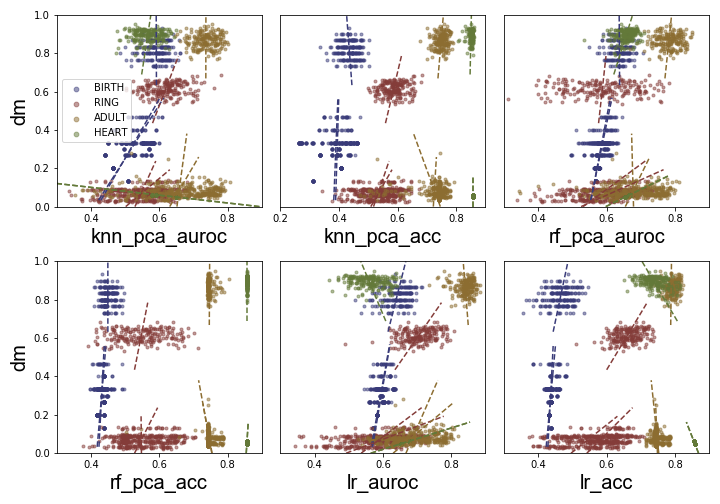
\includegraphics[width=0.8\textwidth]{project/fig/scatter_sep_trends/dm_scatter.png}
    \caption{Scatterplots of the utility measures for the different classifiers against the diameter metric, separated by datasets. For every dataset, we draw a line of best fit per algorithm.}
\end{figure}

\begin{figure}[!ht]
    \centering
    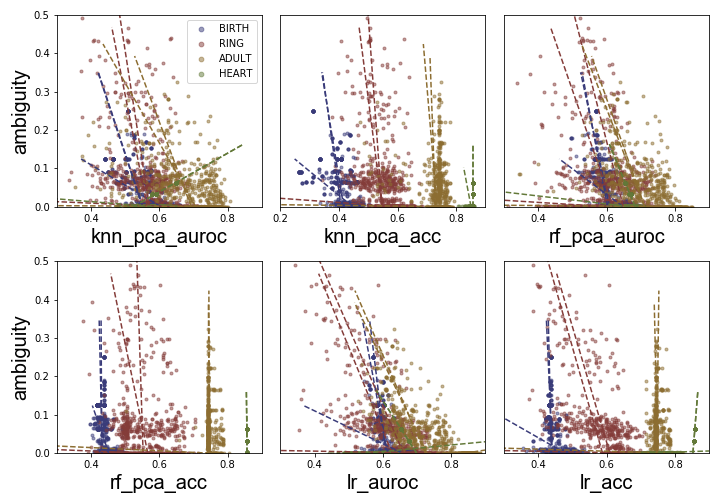
\includegraphics[width=0.8\textwidth]{project/fig/scatter_sep_trends/ambiguity_scatter.png}
    \caption{Scatterplots of the utility measures for the different classifiers against the ambiguity metric, separated by datasets. For every dataset, we draw a line of best fit per algorithm.}
\end{figure}

\begin{figure}[!ht]
    \centering
    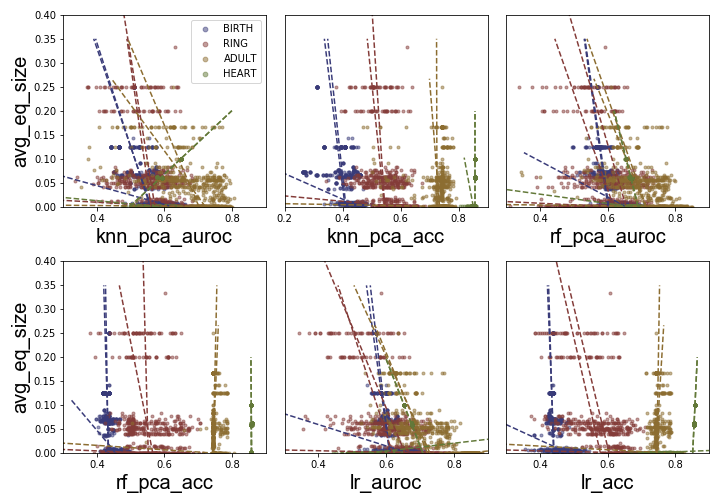
\includegraphics[width=0.8\textwidth]{project/fig/scatter_sep_trends/avg_eq_size_scatter.png}
    \caption{Scatterplots of the utility measures for the different classifiers against the average equivalence class size metric, separated by datasets. For every dataset, we draw a line of best fit per algorithm.}
\end{figure}

\begin{figure}[!ht]
    \centering
    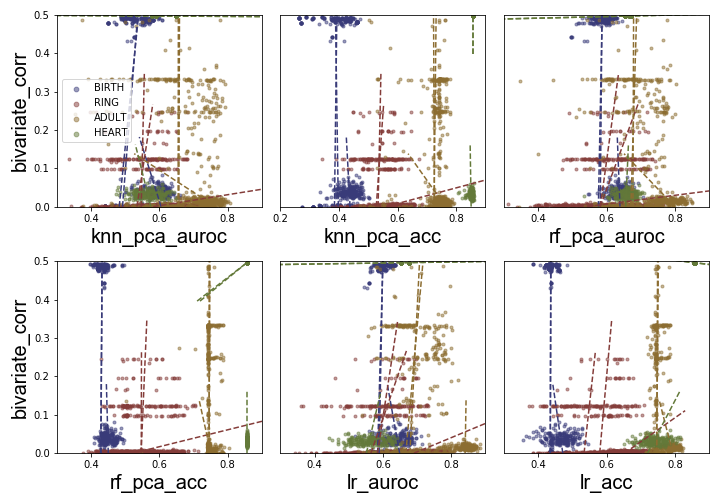
\includegraphics[width=0.8\textwidth]{project/fig/scatter_sep_trends/bivariate_corr_scatter.png}
    \caption{Scatterplots of the utility measures for the different classifiers against the bivariate correlation metric, separated by datasets. For every dataset, we draw a line of best fit per algorithm.}
\end{figure}

\begin{figure}[!ht]
    \centering
    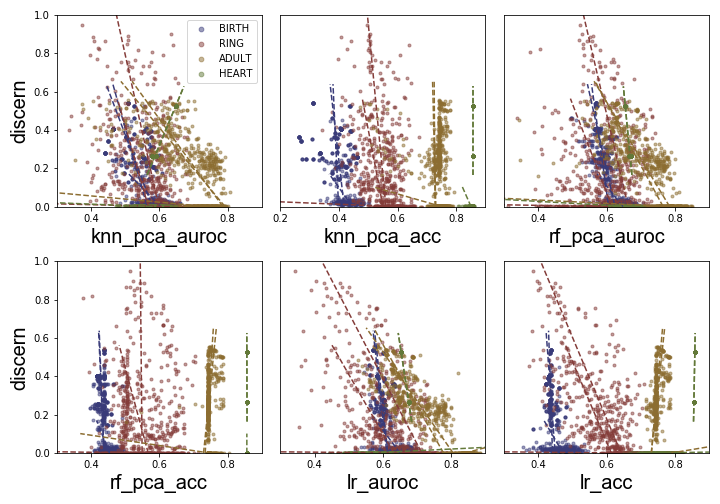
\includegraphics[width=0.8\textwidth]{project/fig/scatter_sep_trends/discern_scatter.png}
    \caption{Scatterplots of the utility measures for the different classifiers against the discernibility metric, separated by datasets. For every dataset, we draw a line of best fit per algorithm.}
\end{figure}

\begin{figure}[!ht]
    \centering
    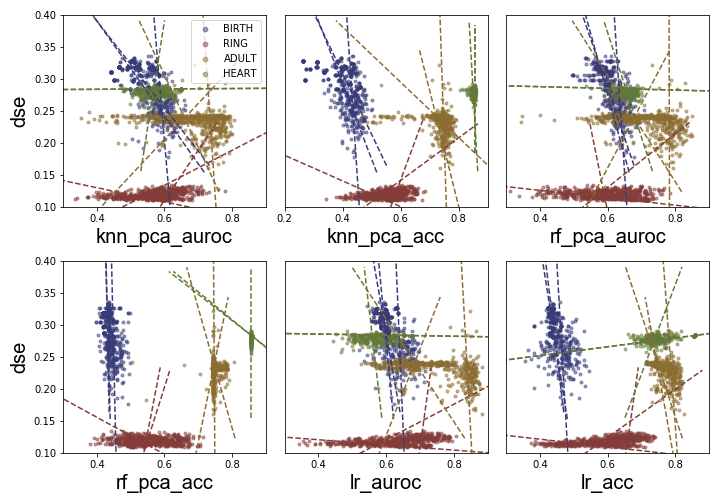
\includegraphics[width=0.8\textwidth]{project/fig/scatter_sep_trends/dse_scatter.png}
    \caption{Scatterplots of the utility measures for the different classifiers against the squared distance error metric, separated by datasets. For every dataset, we draw a line of best fit per algorithm.}
\end{figure}

\begin{figure}[!ht]
    \centering
    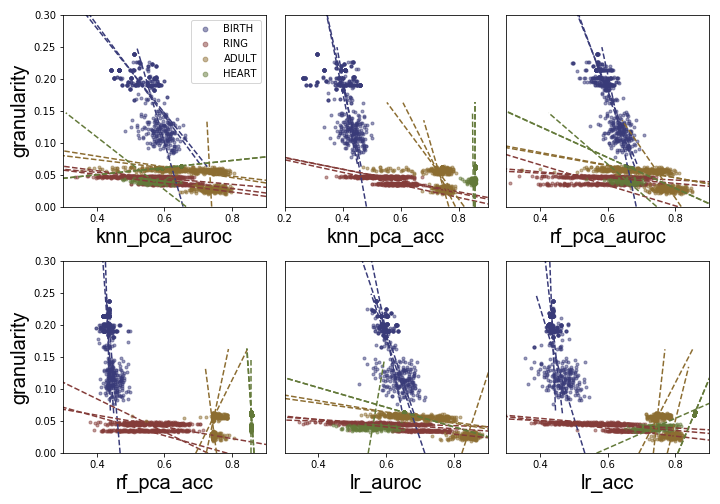
\includegraphics[width=0.8\textwidth]{project/fig/scatter_sep_trends/granularity_scatter.png}
    \caption{Scatterplots of the utility measures for the different classifiers against the granularity metric, separated by datasets. For every dataset, we draw a line of best fit per algorithm.}
\end{figure}

\begin{figure}[!ht]
    \centering
    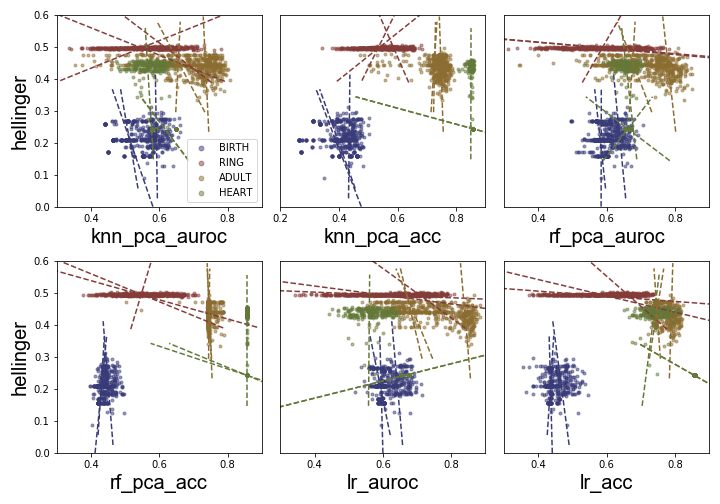
\includegraphics[width=0.8\textwidth]{project/fig/scatter_sep_trends/hellinger_scatter.png}
    \caption{Scatterplots of the utility measures for the different classifiers against the hellinger metric, separated by datasets. For every dataset, we draw a line of best fit per algorithm.}
\end{figure}

\begin{figure}[!ht]
    \centering
    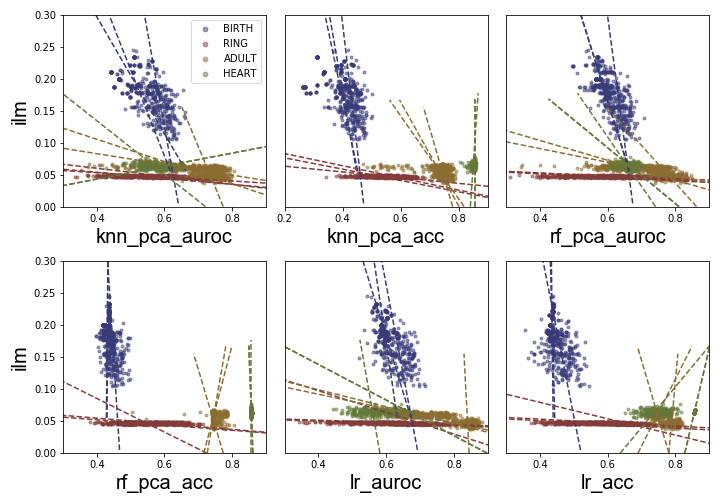
\includegraphics[width=0.8\textwidth]{project/fig/scatter_sep_trends/ilm_scatter.png}
    \caption{Scatterplots of the utility measures for the different classifiers against the information loss metric, separated by datasets. For every dataset, we draw a line of best fit per algorithm.}
\end{figure}